%%%%% this line is 80 chars wide, please don't make longer lines %%%%%%%%%%%%%%%

\subsection{Rate modulation depth}

\begin{figure*}[ht]
	\centering
  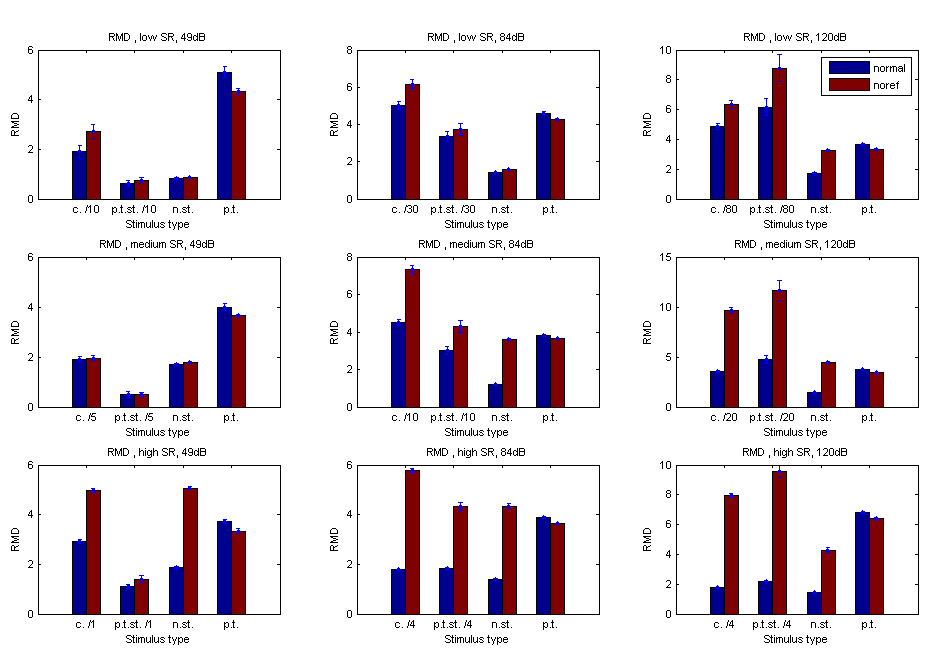
\includegraphics[width=0.75\textwidth]{images/rmds9.jpg}
	\caption{RMD values for different SR fibers and intensities}
	\label{fig:rmds}
\end{figure*}

For the first part of the project, an ad-hoc calculation called rate 
modulation depth (RMD) was used to see difference between encoding 
of acoustic signal with and without absolute refractory period (ARP).

Four kinds of experiments where run and the means of RMD was calculated 
for each of them, 
with each type of nerve fiber, and three different intensities : 
49dB SPL, 84dB SPL and 120dB SPL to have an overall view of effects. 
For every experience, the bin size was 0.01 ms, the characteristic frequency was 1 kHz, 
there was no damage on IHC or OHC, and we told the model to use approximations 
for power-law function calculations. No noise was added to the stimuli.

The four experiments were clicks, pure tones, noise steps and pure tone steps.
The clicks were rarefaction clicks of 0.1 ms and sufficient time was waited between 
two of them to avoid influence from one to the other.
The two steps stimuli had a period of 100 ms and in the first half of the period 
there was noise or pure tone signal, and in the second half there was 0 Pa as pressure.
The noise for the noise step was composed of random normal variables divided 
by the square root of the bin size (gaussian white noise).
The pure tone of the pure tone step was of 10kHz frequency.

We computed then RMD like that : 

$(max - baseline) / baseline$,

where max was 
the maximum of the periodogram of the encoded sounds when converted in 2 ms bins.
The meaning of the baseline depended on the stimulus. 
For the clicks it corresponded to the response of a 0 Pa pressure signal, 
for the noise step it was the value of the periodogram just before the second 
half of the period, in 10 ms bins. 
The baseline for the pure tone step was the mean of value of periodogram 
of a response to a pure tone of the frequency used for the stimulus (10 kHz),
after the IHC were saturated and have no time to be depolarized. 
It was seen in experiments that 0.02 ms were sufficient to attain saturation,
so for the baseline the first 0.02 ms were not used.
For the pure tone, the baseline was chosen as the mean of the periodogram.
When baselines for clicks and for pure tone step where computed, 
we took attention to the fact that the number of repetitions of stimulus
for the used periodogram should correspond to the one for the periodogram used for 
calculating the maximum. 
It gives then an equivalent RMD as if we had divided each periodogram by 
their own number of repetitions.

As you can see on \autoref{fig:rmds}, for each type of nerve fiber and 
each decibel value experimented we have similar values in this sense :
for clicks, pure tone steps and noise steps, the RMD without absolute refractory
period is bigger than the normal case, and it is the opposite for pure tones.

%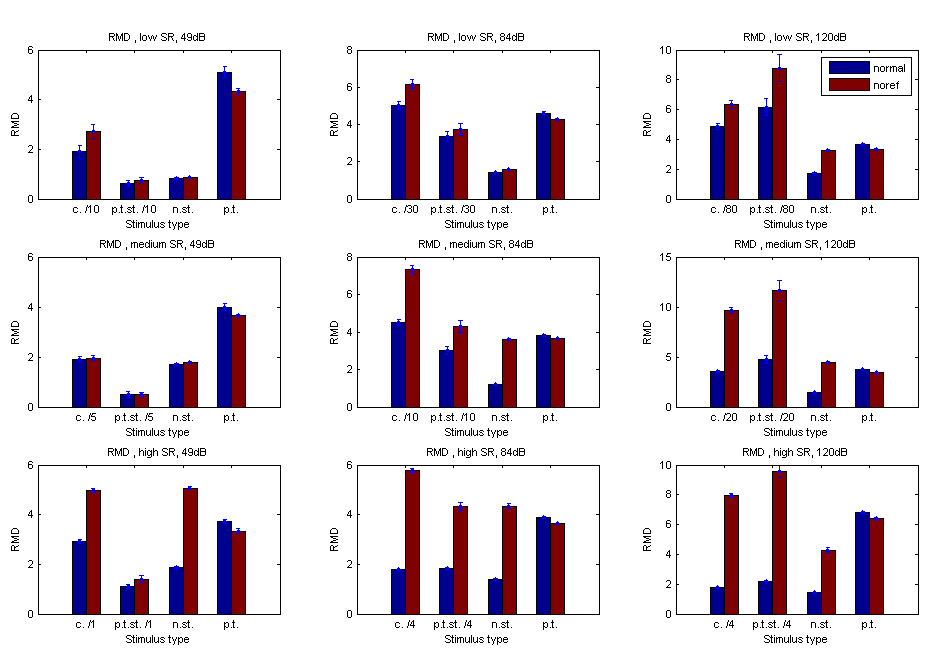
\includegraphics[width=0.45\textwidth]{images/rmds9.jpg}


We probably can explain the first fact because first, we are in presence of a highly 
non-linear system and, 
secondly, the three stimuli for which the RMD without ARP is bigger than with 
ARP are stimuli with sudden changes. 
In fact, the click can be seen as an approximation of a delta function, 
and for the steps we have suddenly a signal for some time and suddenly, 
we have no more of it, and that repeatedly. % so ...... ?

The second fact, the fact that RMD is lower for pure tones without ARP, 
corresponds to what can % ....... ?

\subsection{Response according to frequencies of modulated pure tones}

In \cite{Deger}, predictions are done for norm and angle of Fourier coefficients of 
response of processes with refractory period.
In fact, the mathematical link between $1/d$, $d$ being the absolute refractory period
and the modulation frequency f is of first importance according to the predictions.

%.......?

%image from paper ?





 